\chapter{Problème spectral pour le calcul de $\mathbf{u}$}
On peut maintenant résoudre le problème \ref{fvc} :
\[ \frac{\partial c_k}{\partial t} + \frac{1}{Re}c_k\lambda_k^2 + \sum_{i=1}^M\sum_{j=1}^Mc_ic_jR_{ijk} + \sum_{i=1}^Mc_iR_{iak} + \sum_{i=1}^Mc_iR_{raij} = R_{fk}+R_{pk} \]
où
\begin{align*}
R_{ijk} &= \lambda_i\int_\Omega(\mathbf{g_i}\times \mathbf{g_j})\cdot\mathbf{g_k} & R_{iak} &= \lambda_i\int_\Omega(\mathbf{g_i}\times \mathbf{a})\cdot\mathbf{g_k}\\
R_{raij} &= \int_\Omega((\curl\mathbf{a})\times \mathbf{g_i})\cdot\mathbf{g_k} & R_{fk} &= \int_\Omega\mathbf{f_a}\cdot\mathbf{g_k}\\
R_{pk} &= \int_{\partial\Omega} \alpha_2\phi_k
\end{align*}
Cela nous permet de connaître les coefficients $c_i$ dans la décomposition $\mathbf{u}=\sum_{i=1}^M c_i\mathbf{g_i}$.\\

%% Dans l'état actuel, comme nous n'avons pas encore déterminé comment relever $\alpha_2$, on veut faire porter sa contribution sur $\mathbf{f}$ et donc dans le terme $R_{fk}$. La conséquence est que $\mathbf{a}$ ne relève pas la condition $\curll\mathbf{v}\cdot\mathbf{n}=\alpha_2$, ainsi $\mathbf{a}=\grad\psi^0+\curl\mathbf{b}$.\\

De plus, dans le cylindre, comme $\alpha_1=0$, on a $\mathbf{a}=\grad\psi^0$ et donc comme le rotationnel d'un gradient est nul, $\curl \mathbf{a} = 0$. Ce qui amène le terme $R_{raij}$ à être nul. On a donc plus que :
\[ \frac{\partial c_k}{\partial t} + \frac{1}{Re}c_k\lambda_k^2 + \sum_{i=1}^M\sum_{j=1}^Mc_ic_jR_{ijk} + \sum_{i=1}^Mc_iR_{iak} = R_{fk}+R_{pk} \]

\section{Navier-Stokes}
\label{PSNewton}
Cette équation comporte le terme
\[ \sum_{i=1}^M\sum_{j=1}^M c_i c_jR_{ijk} \]
qui est non linéaire. Ce problème s'écrit donc sous la forme :
\[ F(c) = 0 \]
où $F:\R^M\rightarrow\R^M$, $c=(c_1,\ldots, c_M)$ et :
\begin{equation}\label{psf}
 F_k(c) = \frac{1}{Re} c_k\lambda_k^2 + \sum_i c_i R_{iak} + \sum_{i,j} c_i c_j R_{ijk} - R_{fk} - R_{pk}
\end{equation}

On va utiliser une méthode de Newton pour résoudre ce problème, on cherche donc :
\begin{equation}\label{Newton}
c^{(l+1)} = c^{(l)} - J(c^{(l)})^{-1}F(c^{(l)})\quad l=0,1,\ldots
\end{equation}
où $c^{(0)}$ est une donnée initiale et $J(c)$ est la matrice jacobienne de $F$ en $c$ :
\[ J(c)=
\begin{pmatrix}
\frac{\partial F_1(c)}{\partial c_1} & \ldots & \frac{\partial F_1(c)}{\partial c_M}\\
\vdots & \ddots & \vdots\\
\frac{\partial F_M(c)}{\partial c_1} & \ldots & \frac{\partial F_M(c)}{\partial c_M}
\end{pmatrix}\]
avec 
\begin{equation}\label{psj}
J(c)_{ki} = \frac{\partial F_k(c)}{\partial c_i} = \delta_{ki}\lambda_i^2 + R_{iak} + \sum_j c_j \underbrace{\lambda_i(\mathbf{g_i}\times\mathbf{g_j},\mathbf{g_k})}_{R_{ijk}} + \sum_j c_j\underbrace{\lambda_j (\mathbf{g_j}\times\mathbf{g_i},\mathbf{g_k})}_{R_{jik}}
\end{equation}
avec $\delta_{ki}$ le symbole de Kronecker et où on a inversé le rôle de $i$ et de $j$ dans $R_{jik}$.\\

Résoudre (\ref{Newton}) est équivalent à résoudre 
\begin{align}
J(c^{(l)})\delta c^{(l)} = -F(c^{(l)})\label{INewton1}\\
c^{(l+1)}=c{(l)}+\delta c^{(l)}\nonumber
\end{align}

On itère ce système jusqu'à ce que la différence entre deux itération soit inférieure à une certaine tolérance, c'est-à-dire $||\delta c^{(l)}||<tol$ ou que le nombre d'itération soit trop grand, ce qui indique la non convergence du système.

\subsection{Implémentation}
Comme on va manipuler des matrices pleines, au lieu d'utiliser PETSc, qui est plus adapté aux matrices creuses, on utilise la librairie Eigen \cite{eigenweb}.\\
Dans cette librairie, on déclare une matrice comme \texttt{Matrix<type, ligne, colonne>}. Afin de pouvoir utiliser des matrices de tailles différentes à chaque exécution, on utilise le mot clé \texttt{Dynamic} pour la taille. Il existe un type pré-déclaré pour le type \texttt{Matrix<Double, Dynamic, Dynamic>} : \texttt{MatrixXd}. De même pour le type \texttt{Matrix<Double, Dynamic, 1>}, qui est un vecteur de double de taille variable, on utilise le mot clé \texttt{VectorXd}.\\

Par exemple, si on a un vecteur de la librairie standard contenant les différentes valeurs des $\lambda_i$, on les stock dans un vecteur de la librairie Eigen avec les lignes de code suivantes : 
\lstinputlisting[linerange=lambda]{../../src/spectralproblem.cpp}
où $M$ est le nombre de valeurs propres que l'on a précédemment calculées. On remarque aussi que l'on peut accéder aux éléments du vecteur avec l'opérateur \texttt{()}.\\

Chaque somme de l'équation \ref{fvc} peut être considérée comme un élément de la librairie Eigen. Ainsi $R_{iak}=\lambda_i\int (\mathbf{g_i}\times\mathbf{a})\cdot\mathbf{g_k}$ est un élément d'une matrice, celui de la $i$-ième ligne et $k$-ième colonne.\\
$R_{fk} = \int \mathbf{f_a}\cdot\mathbf{g_k}$ et $R_{pk} = \int_{\partial\Omega}\alpha_2\psi_k$ sont des vecteurs et $R_{ijk} = \lambda_i\int (\mathbf{g_i}\times\mathbf{a})\cdot\mathbf{g_k}$ est un élément en 3 dimensions, donc un vecteur de matrices. On a ainsi les déclarations suivantes :\\
\lstinputlisting[linerange=ri]{../../src/spectralproblem.hpp}

On initialise d'abord la mémoire nécessaire pour contenir le vecteur, puis on initialise chaque élément de la matrice $R_{iak}$ à l'aide de deux boucles imbriquées :\\
\lstinputlisting[linerange={riakInit,riakComp}]{../../src/spectralproblem.cpp}

De même, on initialise la mémoire utilisée par la matrice, puis chaque élément du vecteur $R_{fk}$ avec une boucle :\\
\lstinputlisting[linerange={rfkInit,rfkComp}]{../../src/spectralproblem.cpp}

On procède pareil pour $R_{pk}$ en ayant pris le soin de créer une expression avec $\alpha_2$, rentré en paramètre :\\
\lstinputlisting[linerange={rpkInit,rpkComp}]{../../src/spectralproblem.cpp}

Pour $R_{ijk}$, on doit tout d'abord initialiser le vecteur contenant les matrices, puis pour chaque élément de ce vecteur, initialisé la mémoire de la matrice elle-même. Ensuite seulement, on peut initialiser chaque élément de $R_{ijk}$ :\\
\lstinputlisting[linerange={rijkInit,rijkComp}]{../../src/spectralproblem.cpp}

Afin d'appliquer la méthode de Newton, il faut d'abord initialiser un vecteur pour stocker la solution $\delta c^{(l)}$ au problème \ref{INewton1} et choisir la tolérance pour laquelle on considère le système résolut.\\
\lstinputlisting[linerange=NSInit]{../../src/spectralproblem.cpp}

On peut maintenant appliquer la méthode de Newton décrite dans \ref{PSNewton}. On veut donc exprimer le vecteur $F(c)$ (\ref{psf}) dans la librairie Eigen. On utilise donc le mot clé \texttt{wiseProduct} pour faire un produit élément par élément de $c$ et de $\lambda$, et on multiplie la matrice $R_{iak}$ avec $c$, on retranche aussi le vecteur $R_{fk}$.\\
Puis pour la ligne $k$, le terme non linéaire $\sum_{i,j} c_i\lambda_i c_j (\mathbf{g_i}\times \mathbf{g_j}, \mathbf{g_k})$ est le produit $c^TR_{ijk}(k)c$ où $R_{ijk}(k)$ est la matrice se trouvant à la $k$-ième position dans le vecteur $R_{ijk}$ et $c^T$ est le vecteur transposé de $c$.\\
\lstinputlisting[linerange=NSMatF]{../../src/spectralproblem.cpp}

Pour la matrice $J(c)$ (\ref{psj}), le terme $\delta_{ik}\lambda^2$, signifie que le vecteur $\lambda^2$ se trouve sur la diagonale de $J(c)$, on utilise donc le mot clé \texttt{asDiagonal} pour effectuer cette opération. On ajoute aussi la matrice $R_{iak}$ telle quelle à $J(c)$.\\
Le terme $\sum_j c_j\lambda_j (\mathbf{g_j}\times\mathbf{g_i},\mathbf{g_k})$ est égal au $i$-ième élément du vecteur produit $c^TR_{ijk}$, tandis que $\sum_j\lambda_i c_j (\mathbf{g_i}\times\mathbf{g_j},\mathbf{g_k})$ est le $i$-ième élément du vecteur $c^TR_{ijk}^T$, car $R_{jik}=R_{ijk}^T$.\\
\lstinputlisting[linerange=NSMatJ]{../../src/spectralproblem.cpp}

Il faut aussi initialiser le solveur avec lequel résoudre les systèmes \ref{INewton1}, par exemple, pour les résoudre avec une méthode de Householder, on utilisera les lignes suivantes :\\
\lstinputlisting[linerange={NSSys1,NSSys2}]{../../src/spectralproblem.cpp}

Il suffit maintenant d'additionner $c^{(l)}$ et $c^{(l+1)}$ pour obtenir la solution à l'itération suivante.\\
\lstinputlisting[linerange=NSAdd]{../../src/spectralproblem.cpp}

On itère ces étapes jusqu'à ce que la tolérance soit dépassée, ou que l'on pense que la méthode diverge.

\section{Stokes}
\label{stokes}
Si l'on supprime le terme non linéaire et que l'on se place dans un cas stationnaire, l'équation du problème \ref{depart} devient :
\begin{equation}\label{stokesEq} \grad q + \curll\mathbf{v} = \mathbf{f} \end{equation}
Or $q = \frac{\mathbf{v}\cdot\mathbf{v}}{2} + p$, et $\mathbf{v}\cdot\mathbf{v}\restr{\Gamma}=\alpha_0^2$, d'où $\grad q\restr{\Gamma} = (\partial_x(\alpha_0^2), \partial_y(\alpha_0^2), \partial_z(\alpha_0^2)) + \grad p\restr{\Gamma} =  \grad p\restr{\Gamma}$.\\
De plus, pour un écoulement de Poiseuille dans un cylindre, on a : \[ v_{max} = \frac{R^2}{4\nu}\left\lvert\frac{\partial p}{\partial z}\right\rvert \mbox{ d'où } \left\lvert\frac{\partial p}{\partial z}\right\rvert = v_{max}\frac{4\nu}{R^2} \]
Or, dans un écoulement de Poiseuille, la pression est linéaire et dépendante uniquement de $z$. On a donc que \[ \grad p = ( 0, 0, \partial_z p) = (0,0,\pm v_{max}\frac{4\nu}{R^2}) \]
Le problème ayant été adimensionnalisé, on a $v_{max}=2,\, R=0,5\mbox{ et } \nu=1$, de plus, on veut que l'écoulement soit dans le sens positif, donc que $p$ soit décroissant.\\
On a donc :
\[ \grad p = (0,0, 32) \]
En prenant la composante normale de l'équation (\ref{stokesEq}), on obtient :
\[ \alpha_2 = \curll\mathbf{v}\cdot\mathbf{n}\restr{\Gamma} = \mathbf{f}\cdot\mathbf{n}\restr{\Gamma} - \grad p\cdot\mathbf{n}\restr{\Gamma} = \begin{cases} 31 & \mbox{ sur } \Gamma_1\\ -31 & \mbox{ sur } \Gamma_2\\ 0 & \mbox{ sur }\Gamma_3\end{cases} \]

\subsection{Implémentation}
L'équation du problème \ref{fvc} s'écrit alors :
\[ \sum_i c_iR_{iak} +\frac{1}{Re}c_k\lambda^2 = R_{fk} + R_{pk} \]

Ainsi, il suffit de résoudre l'équation $Ax=b$ où $A=(a_{ki})$ avec :
\[ a_{ki} = \delta_{ki}\frac{\lambda^2}{Re} + R_{iak} \]
et
\[ b_k = R_{fk} + R_{pk} \]

Il faut donc créer la matrice $A$ à l'aide des $\lambda$ et de $R_{iak}$ :\\
\lstinputlisting[linerange=StokesA]{../../src/spectralproblem.cpp}
et le vecteur $b$ avec $R_{fk}$ :\\
\lstinputlisting[linerange=StokesB]{../../src/spectralproblem.cpp}

Puis, on résout le système de la même manière que précédemment :\\
\lstinputlisting[linerange=StokesSolve]{../../src/spectralproblem.cpp}

\subsection{Résultats}
Dans la figure \ref{vitesse}, on voit la vitesse $\mathbf{v}=\mathbf{a}+\mathbf{u}$ obtenue en utilisant $\mathbf{f}=(0,0,1)$, correspondant à la gravité adimensionnalisée, et $\alpha_2$ tel que défini dans \ref{stokes}.
\begin{figure}[H]
  \makebox[\textwidth][c]{
    \subfloat[écoulement au centre]{\label{vGradPression}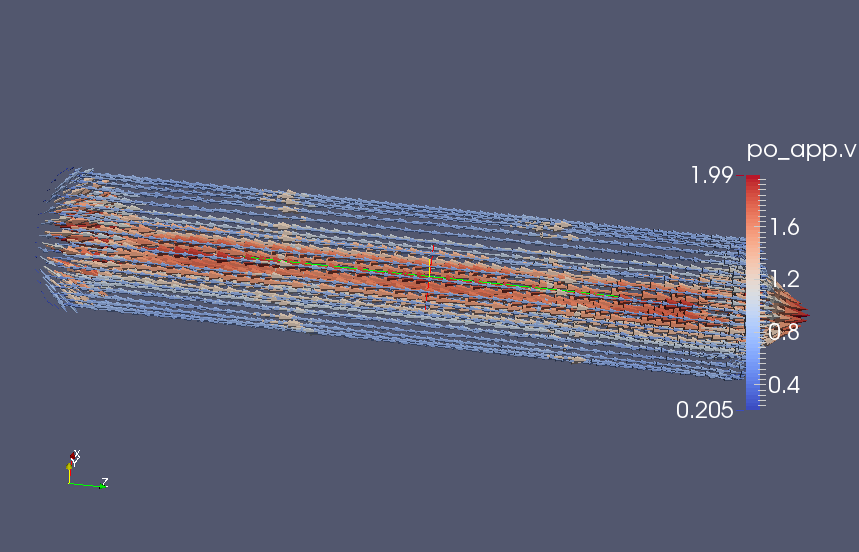
\includegraphics[scale=0.3,trim=0mm 0mm 0mm 11mm,clip]{vGradPression32-32}}\ 
    \subfloat[magnitude dans le plan]{\label{v100modes}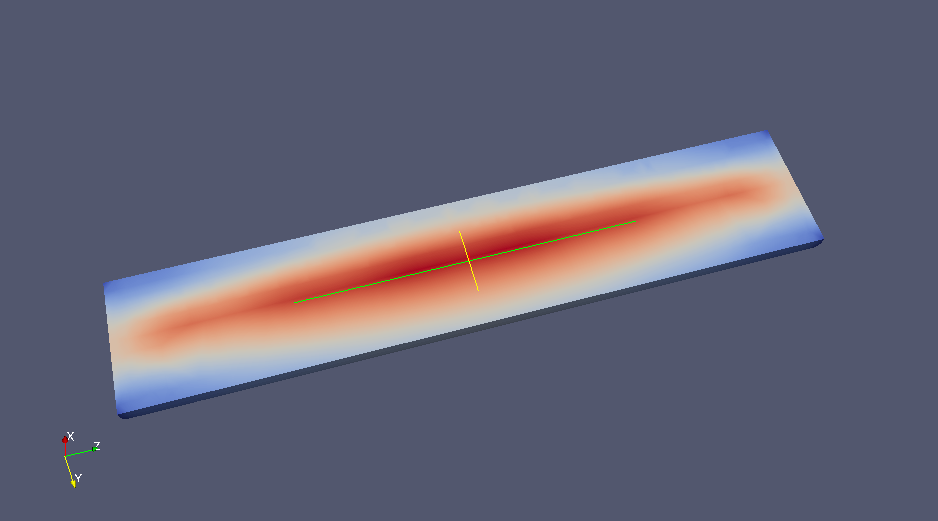
\includegraphics[scale=0.3]{v100modes}}
  }
\caption{Vitesse dans le cylindre}\label{vitesse}
\end{figure}

Les résultats ci-dessus ont été obtenus avec 50 modes et 3 processeurs, on voit d'ailleurs dans la figure \ref{vGradPression} qu'aux mailles correspondantes à la jointure des partitions, le champ n'est pas régulier. Cela peut être dû au faible nombre de mailles utilisé.\\
L'image \ref{v100modes} montre que l'écoulement n'est pas exactement un écoulement de Poiseuille, la vitesse dépendant de $z$, et les composantes $\mathbf{v}_x$ et $\mathbf{v}_y$ n'étant pas tout à fait nulles. Cependant, comme le montre la figure \ref{tendto}, on peut voir que cela est dépendant du nombre $M$ de modes utilisés, plus ce nombre est grand plus ce phénomène tend à disparaître.\\

\begin{figure}[H]
	\makebox[\textwidth][c]{
      \subfloat[M=10]{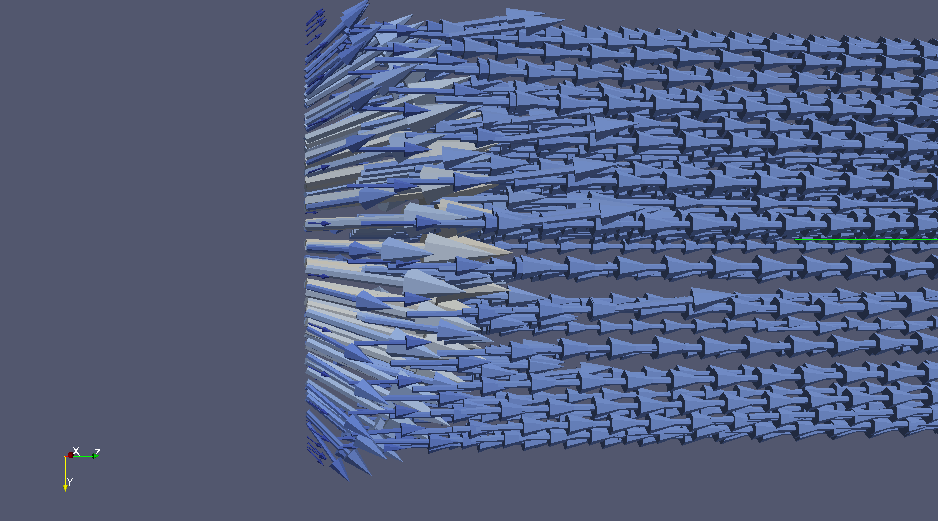
\includegraphics[scale=0.5,trim=100mm 20mm 100mm 20mm,clip]{vIn10}}\ 
		\subfloat[M=100]{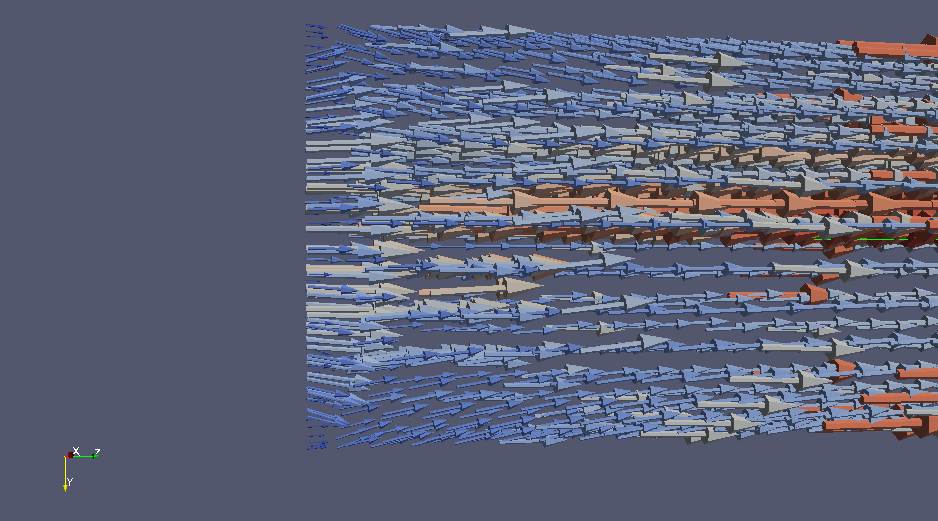
\includegraphics[scale=0.5,trim=100mm 20mm 100mm 20mm,clip]{vIn100}}
	}
\caption{Composantes $x$ et $y$ à l'entrée du cylindre}\label{tendto}
\end{figure}

\subsection{Temps de calcul}
La figure \ref{histo} montre le temps de calcul pour les différentes étapes du problème. Les étapes sont :
\begin{enumerate}
\item Eigen : trouver les modes propres (problème \ref{disceigenh1})
\item Decomp : décomposer les fonctions propres (problèmes \ref{fvgi0} et \ref{fvpsiml})
\item Riak : calculer la matrice $R_{iak}$ pour $i,k=1,\dots,M$
\item Rfk : calculer le vecteur $R_{fk}$ pour $k=1,\dots,M$
\item Rpk : calculer le vecteur $R_{pk}$ pour $k=1,\dots,M$
\item Stokes : résoudre le problème de Stokes
\end{enumerate}
Ces tests ont été effectué sur le cluster \texttt{irma-hpc2}, équipé de 24 processeurs AMD Opteron cadencés à 2812 MHz et 110 GB de RAM, mais en utilisant seulement 10 processeurs.\\

On peut voir que si pour un faible nombre de modes propres, le problème aux valeurs propres est ce qui coûte le plus de temps, dès que ce nombre accroît, la partie la plus chère en temps de calcul est la détermination des coefficients $R_{iak}$.\\
De plus, dans le problème de Stokes, on a supprimé le besoin de calculer les coefficients $R_{ijk}$, alors que ce sont ces coefficients qui doivent prendre le plus de temps de calcul. En effet, si pour $R_{fk}$ et $R_{pk}$ on doit calculer $M$ coefficients, pour $R_{iak}$, il y a $M^2$ coefficients et pour $R_{ijk}$, il y a $M^3$ coefficients à calculer.\\
Pour $M=100$, on a donc $10300$ coefficients à calculer pour le problème de Stokes, contre $1010300$ pour Navier-Stokes.

\begin{figure}[H]
\centering
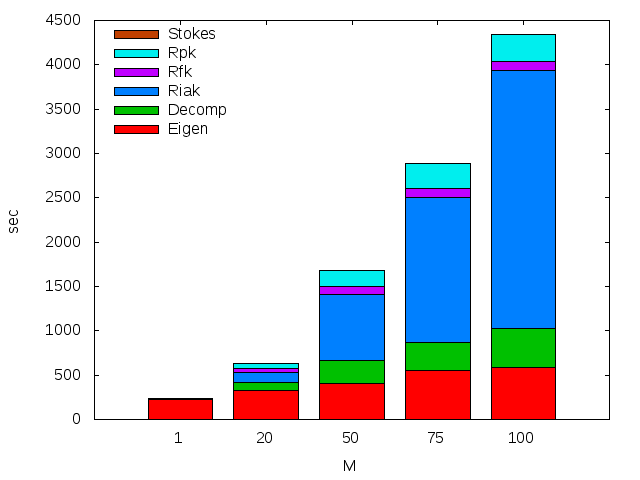
\includegraphics[scale=0.9]{histo}
\caption{Temps de calcul des différentes étapes du problème}\label{histo}
\end{figure}


%%% Local Variables:
%%% TeX-master: "../report.tex"
%%% eval: (flyspell-mode 1)
%%% ispell-local-dictionary: "french"
%%% End:
